\uuid{6988}
\titre{Exercice 6988}
\theme{}
\auteur{blanc-centi}
\date{2015/07/04}
\organisation{exo7}
\contenu{
  \texte{}
  \question{Trouver les droites à la fois tangentes et orthogonales à la courbe 
$$\left\{\begin{array}{l}x(t)=3t^2\\ y(t)=4t^3\end{array}\right.$$}
  \reponse{\begin{enumerate}
  \item Commençons par trouver le vecteur tangent à la courbe au point $M(t)$. 
  Les fonctions $x$ et $y$ sont de classe $\mathcal{C}^1$ sur $\R$, et 
  $x'(t)=6t$, $y'(t)=12t^2$. Si $t\not=0$, le vecteur tangent à la courbe 
  au point $M(t)$ est donc le vecteur dérivé 
  $\begin{pmatrix}6\\ 12t\end{pmatrix}$. Si $t=0$, 
  le vecteur dérivé est nul et il faut dériver encore une fois pour 
  obtenir un vecteur non nul $\begin{pmatrix}x''(0)\\ y''(0)\end{pmatrix}
  =\begin{pmatrix}6\\ 0\end{pmatrix}$, qui est donc un vecteur 
  directeur de la tangente au point $M(0)$. Finalement, pour tout $t$, 
  la tangente au point $M(t)$ est dirigée par le vecteur 
$$\vec{V}=\begin{pmatrix}6\\ 12t\end{pmatrix}$$  

  \item 
\begin{itemize}
  \item Une droite $D$ est tangente à $\mathcal{C}$ s'il existe $t\in\R$ tel 
que $M(t)\in D$ et $\vec{V}(t)$ soit un vecteur directeur de $D$.
  
  \item Une droite $D$ est orthogonale à $\mathcal{C}$ s'il existe $t'\in\R$ tel que $M(t')\in D$ 
et $\vec{V}(t')$ soit un vecteur orthogonal à la droite $D$. 
\end{itemize}


  \item On cherche donc à quelle condition $\vec{V}(t)$ et $\vec{V}(t')$ sont orthogonaux:
$$\vec{V}(t)\cdot\vec{V}(t')=0\Longleftrightarrow 36+144tt'=0\Longleftrightarrow tt'=-\frac{1}{4}$$
ce qui exclut le paramètre $t=0$. 

  \item Soit donc $t\not=0$, et $T(t)$ la tangente à $\mathcal{C}$ en $M(t)$:
$$T(t)=\big\{M(t)+\lambda\vec{V}(t)\ |\ \lambda\in\R\big\}=\left\{\begin{pmatrix}x\\ y\end{pmatrix}\ |\ \exists\lambda\in\R,\ \begin{array}{|l}x=3t^2+6\lambda\\ y=4t^3+12\lambda t\end{array}\right\}$$
En éliminant $\lambda$, on trouve que $T(t)$ a pour équation cartésienne 
$$y=4t^3+2t(x-3t^2)=2tx-2t^3$$

  \item On sait déjà que $T(t)$ et $T(-\frac{1}{4t})$ sont perpendiculaires. Il reste à voir si $T(t)$ coupe bien $\mathcal{C}$ au point $M(-\frac{1}{4t})$:
\begin{eqnarray*}
M\left(-\frac{1}{4t}\right)\in T(t)&\Longleftrightarrow& 4\left(-\frac{1}{4t}\right)^3=2t\cdot 3\left(-\frac{1}{4t}\right)^2-2t^3\\
 &\Longleftrightarrow& 32t^6-6t^2-1=0\\
 &\Longleftrightarrow& X=t^2\quad\mathrm{et}\quad X^3-\frac{3}{16}X-\frac{1}{32}=0
\end{eqnarray*}
L'étude des variations du polyn\^ome $X^3-\frac{3}{16}X-\frac{1}{32}$ montre qu'il admet $-\frac{1}{4}$ comme racine (double), il se factorise donc sous la forme $X^3-\frac{3}{16}X-\frac{1}{32}=(X+\frac{1}{4})^2(X-\frac{1}{2})$ et sa seule racine positive est $\frac{1}{2}$:
\begin{eqnarray*}
M\left(-\frac{1}{4t}\right)\in T(t)&\Longleftrightarrow& X=t^2\quad\mathrm{et}\quad X\in\left\{-\frac{1}{4};\frac{1}{2}\right\}\\
 &\Longleftrightarrow& t^2=\frac{1}{2}\Longleftrightarrow t=\pm\frac{\sqrt{2}}{2}
\end{eqnarray*}

  \item 
Ainsi $T(\frac{\sqrt{2}}{2})$ et $T(-\frac{\sqrt{2}}{2})$ sont les seules 
droites à la fois tangentes et orthogonales à $\mathcal{C}$ :

\begin{itemize}
  \item La droite 
$$T(\frac{\sqrt{2}}{2}):\ y=\sqrt{2}\,x-\frac{\sqrt{2}}{2}$$
est tangente au point $M(\frac{\sqrt{2}}{2})$ et orthogonale au point $M(-1/(4\frac{\sqrt{2}}{2}))$.
  
  \item La droite 
$$T(-\frac{\sqrt{2}}{2}):\ y=-\sqrt{2}\,x+\frac{\sqrt{2}}{2}$$
est tangente au point $M(-\frac{\sqrt{2}}{2})$ et orthogonale au point $M(1/(4\frac{\sqrt{2}}{2}))$.
\end{itemize}

\end{enumerate}

\begin{center}
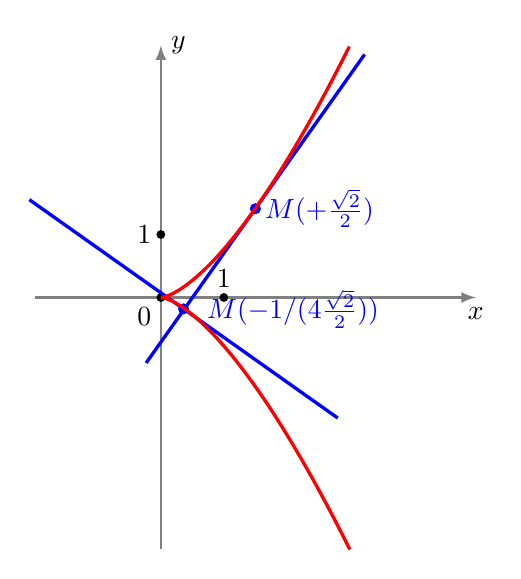
\begin{tikzpicture}[scale=0.80]
     \draw[->,>=latex,thick, gray] (-2,0)--(5,0) node[below,black] {$x$};
     \draw[->,>=latex,thick, gray] (0,-4)--(0,4) node[right,black] {$y$};  


  \fill[black] (0,0) circle (2pt) node[below left]{$0$}; 
  \fill[black] (1,0) circle (2pt)  node[above]{$1$}; 
  \fill[black] (0,1) circle (2pt)  node[left]{$1$}; 


  \coordinate (M1) at (3/2,1.41);
  \fill[blue] (M1) circle (2.5pt)  node[right]{$M(+\frac{\sqrt{2}}{2})$}; 
  \draw[very thick, blue] (M1)--+(54.7:3)--+(54.7:-3);

  \coordinate (MM1) at (0.36,-0.18);
  \fill[blue] (MM1) circle (2.5pt)  node[right=5pt]{$M(-1/(4\frac{\sqrt{2}}{2}))$}; 
  \draw[very thick, blue] (MM1)--+(144.7:3)--+(144.7:-3);

%   \coordinate (M2) at (3/2,-1.41);
%   \fill[green!80!black] (M2) circle (2.5pt)  node[below left=5pt]{$M(-\frac{\sqrt{2}}{2})$}; 
%   \draw[very thick, green!80!black] (M2)--+(-54.7:3)--+(-54.7:-3);
% 
%   \coordinate (MM2) at (0.36,0.18);
%   \fill[green!80!black] (MM2) circle (2.5pt)  node[above]{$M(-\frac{\sqrt{2}}{2})$}; 
%   \draw[very thick, green!80!black] (MM2)--+(-144.7:3)--+(-144.7:-3);

  \draw[red, very thick,domain=-1:1,samples=100] plot ({3*\x*\x},{4*\x*\x*\x});

\end{tikzpicture}  \quad
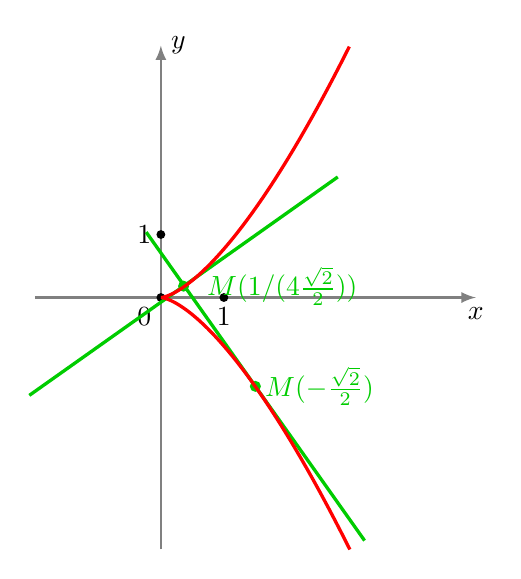
\begin{tikzpicture}[scale=0.80]
     \draw[->,>=latex,thick, gray] (-2,0)--(5,0) node[below,black] {$x$};
     \draw[->,>=latex,thick, gray] (0,-4)--(0,4) node[right,black] {$y$};  


  \fill[black] (0,0) circle (2pt) node[below left]{$0$}; 
  \fill[black] (1,0) circle (2pt)  node[below]{$1$}; 
  \fill[black] (0,1) circle (2pt)  node[left]{$1$}; 


%   \coordinate (M1) at (3/2,1.41);
%   \fill[blue] (M1) circle (2.5pt)  node[right]{$M(+\frac{\sqrt{2}}{2})$}; 
%   \draw[very thick, blue] (M1)--+(54.7:3)--+(54.7:-3);
% 
%   \coordinate (MM1) at (0.36,-0.18);
%   \fill[blue] (MM1) circle (2.5pt)  node[right=5pt]{$M(-1/4\frac{\sqrt{2}}{2})$}; 
%   \draw[very thick, blue] (MM1)--+(144.7:3)--+(144.7:-3);

  \coordinate (M2) at (3/2,-1.41);
  \fill[green!80!black] (M2) circle (2.5pt)  node[right]{$M(-\frac{\sqrt{2}}{2})$}; 
  \draw[very thick, green!80!black] (M2)--+(-54.7:3)--+(-54.7:-3);

  \coordinate (MM2) at (0.36,0.18);
  \fill[green!80!black] (MM2) circle (2.5pt)  node[right=5pt]{$M(1/(4\frac{\sqrt{2}}{2}))$}; 
  \draw[very thick, green!80!black] (MM2)--+(-144.7:3)--+(-144.7:-3);

  \draw[red, very thick,domain=-1:1,samples=100] plot ({3*\x*\x},{4*\x*\x*\x});

\end{tikzpicture} 
\end{center}}
}